\documentclass[conference]{IEEEtran}
\IEEEoverridecommandlockouts

\usepackage[T1]{fontenc}
\usepackage{amsmath,amssymb,mathtools}
\usepackage{booktabs,array}
\usepackage{graphicx}
\usepackage{tikz}
\usetikzlibrary{arrows.meta,positioning,calc}
\graphicspath{{./}{../figures/}}
\usepackage{algorithm}
\usepackage{algpseudocode}
\usepackage{cite}
\usepackage[hidelinks]{hyperref}

\renewcommand{\Pr}{\mathbb{P}}
\newcommand{\kbps}{\,\text{kbps}}

\begin{document}

\title{Choosing a Firewall Rate Threshold Against Flooding Attacks:\\ A Game-Theoretic Study with Independent Flow-Level Checks}

\author{
\IEEEauthorblockN{Maithreya Donthi}
\IEEEauthorblockA{\textit{Dept.\ of Artificial Intelligence}\\
NITK Surathkal\\ 241AI013}
\and
\IEEEauthorblockN{Maharshi Kundu}
\IEEEauthorblockA{\textit{Dept.\ of Artificial Intelligence}\\
NITK Surathkal\\ 241AI022}
\and
\IEEEauthorblockN{Sanskruti Hiwase}
\IEEEauthorblockA{\textit{Dept.\ of Artificial Intelligence}\\
NITK Surathkal\\ 241AI035}
\and
\IEEEauthorblockN{Shriya Bharadwaj}
\IEEEauthorblockA{\textit{Dept.\ of Artificial Intelligence}\\
NITK Surathkal\\ 241AI039}
}

\maketitle

\begin{abstract}
We revisit a one-shot zero-sum model for choosing a firewall rate threshold against flooding attacks. We independently implement its payoff and compare fixed-parameter subgames with published results and a flow-level Monte Carlo simulation. At a fixed attacker mean rate, our subgame saddle points are close to the published values, although we do not reproduce the reported general-game outcome of 120 zombies and payoff 331.1. We identify a mean-times-probability approximation for admitted traffic that can substantially overstate exponential traffic after thresholding. Replacing it with the exact truncated first moment brings the analytical payoffs close to simulation at the selected parameter points we tested. However, the reported best subgame saddle is not generally an equilibrium of the combined game: on our finite grid with the baseline parameters and fixed normal spread, the source and exact-truncated-mean payoff matrices have nonzero minimax gaps. The results therefore support a conditional comparison of subgames, not a pure-strategy equilibrium claim for the full simultaneous game.
\end{abstract}

\begin{IEEEkeywords}
DDoS, flooding attack, firewall, rate limiting, game theory, saddle point, Monte Carlo validation
\end{IEEEkeywords}

%==============================================================
\section{Introduction}
A flooding denial-of-service attack attempts to exhaust a shared resource, such as a network link, by sending more traffic than it can serve. When the traffic originates from many compromised machines, the attack is distributed (DDoS); these machines are commonly called zombies or bots.

Rate limiting is a simple response: a firewall measures each flow's sending rate and drops flows above a selected threshold. A low threshold can reject legitimate users, while a high threshold can admit attack traffic. The choice is therefore a trade-off between service availability and the attacker's admitted bandwidth.

What makes the choice interesting is that the attacker is not a fixed quantity. A rational attacker who knows, or guesses, the threshold will adapt the size of the botnet and the sending rate of each bot, and the defender, anticipating that, will pick the threshold that hurts the attacker most in the worst case. That is the structure of a zero-sum game, and it is the framing used by Spyridopoulos, Karanikas, Tryfonas and Oikonomou~\cite{spyridopoulos2013}, who extend the earlier firewall game of Wu et al.~\cite{wu2010} by letting the attacker choose traffic distribution and rate as well as fleet size.

This paper revisits that model for two reasons. We wanted to understand it well enough to explain each term without hand-waving, and we wanted to know how much of the published numerical story survives an independent implementation. The answer turned out to be more interesting than we expected. Our contributions are the following.
\begin{enumerate}
\item A restatement of the model in a single notation, with explicit closed forms for the probabilities involved and three short derived remarks: the behaviour of the payoff at extreme thresholds, a minimax-gap test for pure-strategy equilibria, and an approximation for the attacker's best fleet size (Section~\ref{sec:model}).
\item An independent implementation of the published nested subgame search and a comparison with the reported fixed-mean and general-search values (Section~\ref{sec:repro}).
\item A flow-level Monte Carlo simulator that draws sender rates and applies the firewall and bottleneck directly. At selected parameter points, it is used to assess the mean-times-probability approximation and an exact-truncated-mean variant (Sections~\ref{sec:mc} and~\ref{sec:exact}).
\item A full-grid maximin/minimax check showing that the nested subgame results do not establish a pure saddle in the combined game, together with a sensitivity analysis of selected subgames (Sections~\ref{sec:repro} and~\ref{sec:sens}).
\end{enumerate}
We propose no new defence mechanism. The contribution is a documented reimplementation and a numerical check of its assumptions. Source code, results and figures are available at \url{https://github.com/Shriyabh11/ddos-firewall-game}.

The rest of the paper is organised as follows. Section~\ref{sec:bg} gives the background and compares related models. Section~\ref{sec:model} presents the game. Section~\ref{sec:reported} summarises the original evidence. Sections~\ref{sec:repro} to~\ref{sec:sens} report our own computations, Section~\ref{sec:disc} discusses them, and Sections~\ref{sec:limits} and~\ref{sec:concl} cover limitations, future work and conclusions.

%==============================================================
\section{Background and Related Work}\label{sec:bg}

\subsection{Flooding attacks and rate limiting}
Flooding attacks work by exhausting a shared resource, usually link capacity or server processing, with traffic that looks like requests. Surveys of DDoS attacks and defences~\cite{mirkovic2004,zargar2013} organise the field along several axes: where the defence is deployed (near the victim, near the sources, or in the middle), when it acts (before, during, or after an attack) and what it relies on (signatures, anomaly detection, rate limiting, puzzles, capacity). Per-flow rate limiting sits in the simplest corner of that taxonomy. It needs only a rate estimate for each flow and a single number, which is why it makes such a clean object for analysis, and also why it cannot tell a heavy but honest user from a slow-and-steady bot.

\subsection{Game-theoretic preliminaries}
Game theory studies decisions where the outcome for each party depends on what the others do. A game specifies the players, the strategies available to each, and a payoff for every combination of strategies. In a \emph{zero-sum} game one player's gain is exactly the other's loss, so a single payoff function $V(a,m)$ describes everything, with one player maximising it and the other minimising it.

Two classical ideas will matter. The first is the minimax principle of von Neumann~\cite{vonneumann1928}: whatever the attacker picks, the defender can guarantee that the payoff is at most $\min_m \max_a V(a,m)$, and the attacker can guarantee at least $\max_a \min_m V(a,m)$. The two guarantees always satisfy
\begin{equation}
\max_{a}\min_{m} V(a,m)\;\le\;\min_{m}\max_{a} V(a,m),
\label{eq:maxmin}
\end{equation}
and equality holds exactly when the game has a pure-strategy \emph{saddle point}, a pair $(a^*,m^*)$ that is simultaneously a best response for both players. The second idea is the Nash equilibrium~\cite{nash1951}, a profile from which no player wants to deviate alone; in two-player zero-sum games the saddle points are the pure Nash equilibria. Textbooks such as Osborne and Rubinstein~\cite{osborne1994} give the details. When no pure saddle exists, equilibrium requires randomisation, which the model we study does not attempt.

Game theory has been widely applied to security problems~\cite{manshaei2013}. A frequent and fair criticism is that attackers are not perfectly rational and that payoff numbers are hard to ground. We return to this in Section~\ref{sec:limits}.

\subsection{Game models of DoS and DDoS defence}
The models in the literature differ mostly in what each player is allowed to do, and that largely determines what they can conclude. Table~\ref{tab:related} summarises the ones most relevant to this paper.

\begin{table}[t]
\caption{Representative game models for DoS/DDoS defence}
\label{tab:related}
\centering\scriptsize
\begin{tabular}{p{0.9cm}p{2.6cm}p{3.2cm}}
\toprule
Work & Defender's move & Attacker's move\\
\midrule
\cite{dingankar2007} & Reconfigure topology & Place zombies in the network\\
\cite{fallah2010} & Choose puzzle-based defence & Attack or not, repeated play\\
\cite{walfish2006} & Ask clients to send more traffic & Flood with full bandwidth\\
\cite{li2009} & Credential caching and detection & Drain verification resources\\
\cite{wu2010} & Firewall rate threshold & Number of zombies\\
\cite{spyridopoulos2013} & Firewall rate threshold & Zombie count, traffic distribution, mean rate, variance\\
\bottomrule
\end{tabular}
\end{table}

Dingankar and Brooks treat the problem as a sequential topology game with no cost attached to moves~\cite{dingankar2007}. Fallah designs puzzle-based defences for an infinitely repeated game, at the price of extra work for every user~\cite{fallah2010}. Walfish et al.\ turn the problem around and encourage honest clients to speak louder, which presumes they have bandwidth to spare~\cite{walfish2006}. Li et al.\ model a different resource altogether, the verification cost in trust-management systems, and show that credential caching shortens the time needed to spot an attacker~\cite{li2009}. Wu et al.\ place a firewall on a dumbbell topology and let the attacker choose how many nodes to use~\cite{wu2010}; the study we follow widens the attacker's options within that same setting~\cite{spyridopoulos2013}.

These results are not directly comparable because the action spaces and cost structures differ. The firewall-threshold game is the narrowest of them, one knob at one place. That narrowness is its main strength as an object of study, and its main limit as a model of real operations.

%==============================================================
\section{The Game Model}\label{sec:model}
This section restates the model of~\cite{spyridopoulos2013}; the structure and equations are theirs, while the closed forms in~\eqref{eq:cdfs}, the exact-truncated-mean variant of Section~\ref{sec:exact} and Remarks~1--3 are ours.

\subsection{Network and traffic}
Figure~\ref{fig:topo} shows the dumbbell topology. $n$ legitimate hosts and $z$ zombies send UDP traffic towards a victim server. A firewall sits in front of a bottleneck link of capacity $BW$. A plain DoS attack is the special case $z{=}1$.

\begin{figure}[t]
\centering
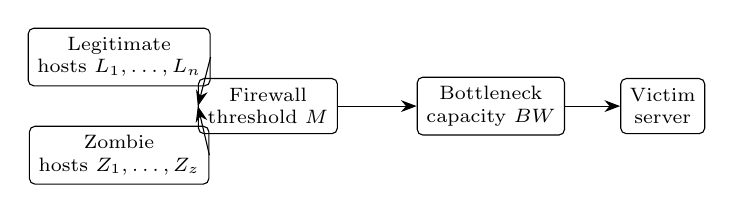
\begin{tikzpicture}[
  node distance=5mm and 7mm,
  box/.style={draw, rounded corners=2pt, minimum height=7mm, font=\scriptsize, align=center},
  arr/.style={-{Stealth[length=2mm]}, thin}]
\node[box] (L) {Legitimate\\hosts $L_1,\dots,L_n$};
\node[box, below=of L] (Z) {Zombie\\hosts $Z_1,\dots,Z_z$};
\node[box, right=10mm of $(L)!0.5!(Z)$] (F) {Firewall\\threshold $M$};
\node[box, right=10mm of F] (B) {Bottleneck\\capacity $BW$};
\node[box, right=7mm of B] (S) {Victim\\server};
\draw[arr] (L.east) -- (F.west);
\draw[arr] (Z.east) -- (F.west);
\draw[arr] (F) -- (B);
\draw[arr] (B) -- (S);
\end{tikzpicture}
\caption{Dumbbell abstraction used by the model. Filtering happens before the shared bottleneck.}
\label{fig:topo}
\end{figure}

Every sender emits at a constant rate that is drawn once from a distribution. Legitimate rates are normal, $F^l_i\sim\mathcal N(f_l,\sigma_l^2)$. Zombie rates $F^z_j$ follow whichever distribution the attacker prefers: normal $\mathcal N(f_z,\sigma_z^2)$, exponential with mean $f_z$, or Poisson with mean $f_z$. These three families are convenient proxies rather than fitted models; the original authors adopt them following~\cite{wu2010}. Capacity is assumed to exceed the total legitimate load, so that any congestion can be blamed on the attack.

The total offered load and the share of each flow that survives congestion are
\begin{equation}
T_B=\sum_{i=1}^{n}F^l_i+\sum_{j=1}^{z}F^z_j,\qquad
\alpha=\min\!\Big(1,\tfrac{BW}{T_B}\Big).
\label{eq:alpha}
\end{equation}
In words, once the link is oversubscribed every flow is scaled down by the same factor. That is a fair-queueing idealisation; it ignores burstiness, retransmissions and queue discipline.

\subsection{Strategies}
The attacker chooses $a=(d,f_z,\sigma_z^2,z)$, with $d$ the distribution family; $\sigma_z^2$ matters only for the normal family. The defender chooses a single threshold $M$. With the hard-threshold rule, a flow whose rate exceeds $M$ is dropped completely and a flow below it is passed. The source also describes a smooth version in which the drop probability follows a sigmoid in the flow rate with midpoint $M$ and steepness $\beta$; as $\beta$ grows it approaches the hard rule, and the published numbers use the hard rule, as do ours.

\subsection{Payoff}
Let $g$ be the lowest rate at which a flow still counts as getting service. Without a firewall, the attacker's share of consumed bandwidth and the fraction of legitimate users pushed below $g$ by congestion are
\begin{align}
V_B &= \frac{z f_z}{n f_l + z f_z}, &
V_U &= \Pr\!\Big(F^l_i<\tfrac{g\,(n f_l + z f_z)}{BW}\Big),
\end{align}
and the attacker's payoff is
\begin{equation}
V=w_b V_B+w_u V_U-w_z\,z,
\label{eq:V}
\end{equation}
where $w_b,w_u,w_z$ weight bandwidth, user loss and per-zombie cost. The defender's payoff is $-V$.

With a hard threshold, flows above $M$ are removed and flows at or below $M$ pass, so the source model's approximate mean admitted rates become
\begin{equation}
f_l'=f_l\Pr(F^l_i\le M),\qquad f_z'=f_z\Pr(F^z_j\le M).
\end{equation}
The attacker's admitted share is $V_B'=z f_z'/(n f_l'+z f_z')$. Legitimate loss now has two sources, congestion and the firewall itself, which the source model adds together:
\begin{equation}
V_U'=\Pr\!\Big(F^l_i<\tfrac{g\,(n f_l'+z f_z')}{BW}\Big)+\Pr\big(F^l_i>M\big).
\label{eq:VU}
\end{equation}
The defended payoff is
\begin{equation}
V'(a,M)=w_b V_B'+w_u V_U'-w_z\,z.
\label{eq:Vp}
\end{equation}
Two cautions apply. Multiplying a mean by a probability is only an approximation to the mean of a truncated distribution, and Section~\ref{sec:exact} shows that the error is large for some attacker families. And the two events in~\eqref{eq:VU} can overlap, so the sum can in principle exceed one; the formula is best read as a score rather than as a probability.

For the closed forms we use in our implementation, let $\Phi$ be the standard normal CDF. Then
\begin{align}
\Pr(F^l_i<x)&=\Phi\!\Big(\tfrac{x-f_l}{\sigma_l}\Big),\notag\\
\Pr(F^z_j\le M)&=\begin{cases}
\Phi\!\big(\tfrac{M-f_z}{\sigma_z}\big) & \text{normal,}\\[2pt]
1-e^{-M/f_z} & \text{exponential,}\\[2pt]
\sum_{k\le\lfloor M\rfloor}\tfrac{e^{-f_z}f_z^{k}}{k!} & \text{Poisson.}
\end{cases}
\label{eq:cdfs}
\end{align}
For the continuous normal and exponential families, the distinction between strict and inclusive thresholds has probability zero. The inclusive convention matters for the discrete Poisson family and is used in the implementation and simulation.

\subsection{Solution concept and search}
A pair $(a^*,M^*)$ is a saddle point of the game if
\begin{align}
V'(a^*,M^*) &\ge V'(a,M^*)\quad\forall a,\\
V'(a^*,M^*) &\le V'(a^*,M)\quad\forall M.
\end{align}
The attacker cannot do better by changing its plan, and the defender cannot reduce the attacker's payoff by moving the threshold. The full simultaneous game has attacker action $a=(d,f_z,\sigma_z^2,z)$ and defender action $M$. The published procedure instead solves a separate $(z,M)$ subgame for each $(d,f_z)$ and reports the subgame saddle with the highest payoff (Algorithm~\ref{alg:search}). This nested scan is useful for reproducing the reported procedure, but it does not in general find a saddle of the combined game: that requires the attacker and defender to use best responses over their entire action spaces at the same pair. We therefore call its outputs \emph{best subgame saddles}, and separately test the combined finite game below.

\begin{algorithm}[t]
\caption{Nested scan of fixed-parameter subgames}
\label{alg:search}
\begin{algorithmic}[1]
\For{each distribution $d$ and mean rate $f_z$}
  \State Build the payoff matrix $V'$ over the grid of $(z,M)$
  \State Mark entries that are column-maximal and row-minimal
  \State Keep the saddle with the largest payoff, if one exists
\EndFor
  \State \Return the highest-payoff subgame saddle (if any)
\end{algorithmic}
\end{algorithm}

\subsection{Three remarks}
\textbf{Remark 1 (extreme thresholds).} As $M\to 0$ nearly every flow is dropped, $\Pr(F^l_i>M)\to1$, and therefore $V'\to w_u-w_z z$, which is largest at $z{=}0$. The attacker is credited with the full user-loss term without sending anything. This is not a bug in the arithmetic, it is what the zero-sum scoring says: users locked out by the defender's own filter count as the attacker's gain. Any sensible defender stays far from this region, but it explains why the payoff surface is steep on the left in Fig.~\ref{fig:br}.

\textbf{Remark 2 (a test for pure saddles).} By~\eqref{eq:maxmin}, a pure saddle exists exactly when the maximin and minimax values coincide. On a discrete grid we can compute both and report the gap. We use the exact saddle test in our search, and use the gap only for diagnosis: in our runs the gap is zero where a saddle exists (for example exponential traffic at $f_z{=}60$ and $120$) and small, about 0.2, in a case without one (normal traffic at $f_z{=}100$), which suggests that near the boundary of existence the failure comes from grid discreteness as much as from true cycling.

\textbf{Remark 3 (an approximate best fleet size).} Write $a=f_z'$ and $b=n f_l'$ for the admitted per-zombie rate and the admitted legitimate load. Then $V_B'=za/(b+za)$ and $\mathrm{d}V_B'/\mathrm{d}z=ab/(b+za)^2$. If we ignore the congestion term in $V_U'$ (it depends on $z$ only weakly), the first-order condition $w_b\,ab/(b+za)^2=w_z$ gives
\begin{equation}
z^{\dagger}\;\approx\;\frac{1}{a}\left(\sqrt{\frac{w_b\,a\,b}{w_z}}-b\right).
\label{eq:zstar}
\end{equation}
For the parameters of Section~\ref{sec:repro} and a normal attacker at $f_z{=}60$, $M{=}119$ this gives $z^\dagger\approx49$, against 55 from the full search; for exponential traffic at $f_z{=}120$, $M{=}95$ it gives about 50 against 57. The estimate is low because congestion loss adds a little marginal benefit for each extra zombie, but it shows the key scaling: the best fleet shrinks roughly like $w_z^{-1/2}$ as the per-host cost rises, and grows with the legitimate load the attacker is competing against.

%==============================================================
\section{What the Original Study Reports}\label{sec:reported}

\subsection{Analytical example}
The analytical example in~\cite{spyridopoulos2013} uses $n{=}80$ legitimate users, $f_l{=}50$~kbps with a spread parameter of 20, $BW{=}5$~Mbps and $g{=}10$~kbps. The weights are $w_b{=}w_u{=}1000$ and $w_z{=}5$, which the authors describe as hypothetical. The search covers $1\le M\le150$~kbps, $0\le z\le120$ and $1\le f_z\le120$~kbps, with a bounded variance range for the normal attacker. Table~\ref{tab:reported} lists what they report.

\begin{table}[t]
\caption{Equilibria reported in the original analytical study}
\label{tab:reported}
\centering\footnotesize
\begin{tabular}{lccc}
\toprule
Setting & $z^*$ & $M^*$ (kbps) & Payoff\\
\midrule
Normal, $f_z{=}60$ & 55 & 119 & 215.4\\
Exponential, $f_z{=}60$ & 53 & 101 & 171.8\\
Poisson, $f_z{=}60$ & 55 & 150 & 215.4\\
Best normal over $f_z$ & -- & -- & 243\\
Best Poisson over $f_z$ & -- & -- & 246.3\\
Normal, $\sigma_z^2$ varied & -- & -- & 255\\
\textbf{General (exp., $f_z{=}120$)} & \textbf{120} & \textbf{96} & \textbf{331.1}\\
\bottomrule
\end{tabular}
\end{table}

Three qualitative claims accompany the numbers. Not every distribution has a pure equilibrium at every mean rate (the normal family has none for $68\le f_z\le84$). The attacker's preferred distribution changes with $f_z$, and for large $f_z$ the exponential is best. And at higher payoff weights or thresholds the attacker's best fleet size moves, which is the role of the cost term.

\subsection{ns-2 validation}
For validation the authors use an ns-2 dumbbell with 80 legitimate UDP senders and a variable number of attack senders. Both groups draw constant rates from normal distributions with means 50 and 60~kbps. The bottleneck is 5~Mbps, packets are 1~kB, and a custom firewall module drops all packets from any node whose configured rate exceeds $M$. They sweep $z\in\{10,\dots,120\}$ and $M\in\{10,\dots,140\}$~kbps, 168 combinations in all, read the trace files to count lost legitimate users and attacker bandwidth, and combine them with the same weights. The reported optimum is about $z{=}50$, $M{=}90$~kbps, payoff about 170.6, which the authors describe as a good approximation to the analytical normal subgame.

\subsection{What each experiment supports}
The ns-2 study uses a normal attacker with fixed mean 60~kbps, so it is a check on the normal $f_z{=}60$ row and on nothing else. It does not test the exponential general-game result. The published description also leaves out the number of random seeds, any confidence intervals, and whether the sender-rate draws were reused across thresholds. The comparison between 119 and 90~kbps, and between 215.4 and 170.6, should therefore be read as qualitative agreement. In Section~\ref{sec:repro} we show that part of the threshold gap is expected, because the analytical payoff is nearly flat over that range.

%==============================================================
\section{Implementation and Reproduction of the Analytical Game}\label{sec:repro}

\subsection{Implementation}
We implemented the game as a small Python package (NumPy and SciPy). The payoff of every $(z,M)$ cell is evaluated in one vectorised call using the closed forms in~\eqref{eq:cdfs}. A saddle point is an entry that is maximal in its column and minimal in its row, with a numerical tolerance of $10^{-9}$; when several saddles exist the one with the highest attacker payoff is kept. The general search loops over distribution families and over $f_z\in\{1,\dots,120\}$~kbps. The grid is every integer $z\in[0,120]$ and $M\in[1,150]$~kbps. Parameters are those of Section~\ref{sec:reported}, and the code is covered by unit tests that check, for example, the low-threshold limit of Remark~1 and that a saddle implies a zero minimax gap.

\emph{On the spread parameter.} The source writes the spread as ``20'', once as a variance and once in kbps. A standard deviation of $\sqrt{20}\approx4.5$~kbps gives equilibrium payoffs between about 48 and 83, nowhere near the published 171 to 215, while a standard deviation of 20~kbps reproduces the published scale. We therefore use 20~kbps for both legitimate and normal zombie traffic.

\subsection{Fixed-mean subgames}
Table~\ref{tab:repro} compares our source-model equilibria at $f_z{=}60$~kbps with the published ones.

\begin{table}[t]
\caption{Fixed-mean subgames ($f_z{=}60$): reported vs.\ our implementation of the source model, as $(z^*,M^*,\text{payoff})$}
\label{tab:repro}
\centering\scriptsize
\begin{tabular}{lccc}
\toprule
 & Normal & Exponential & Poisson\\
\midrule
Reported & (55,119,215.4) & (53,101,171.8) & (55,150,215.4)\\
Ours & (55,114,215.3) & (51,101,167.4) & (55,150,215.4)\\
\bottomrule
\end{tabular}
\end{table}

The Poisson row matches to the first decimal and the other two agree closely in fleet size and payoff. The normal-traffic threshold differs (114 against 119~kbps), but that is not a real disagreement: with $z{=}55$ fixed, our payoff is 215.3 for every integer threshold from 110 up to about 130, so the minimiser is decided in the second decimal. A flat region like this means the model says little about the exact threshold inside it.

\subsection{Nested scan across attacker parameters}
Allowing the attacker mean rate to vary gives the nested scan described above. Table~\ref{tab:general} compares the highest-payoff subgame saddle for each family with the corresponding published value; these entries are not equilibria of the combined simultaneous game. Under our source-model interpretation, the best exponential subgame saddle has 57 zombies and payoff 255.3, rather than the reported 120 zombies and 331.1; its threshold is close (95 against 96~kbps). Evaluating the reported configuration itself (exponential traffic at $f_z{=}120$, $z{=}120$, and $M{=}96$) gives 172.7 under our implementation. We do not know the cause of this discrepancy. Possible explanations include a different parameterisation of the exponential distribution, a different treatment of congestion, or details of the original Matlab routine not specified in the article. We report the discrepancy without claiming to have resolved it.

\begin{table}[t]
\caption{Highest-payoff subgame saddles in the nested scan: reported values vs.\ our source and exact-truncated-mean variants}
\label{tab:general}
\centering\scriptsize\setlength{\tabcolsep}{3pt}
\begin{tabular}{lccc}
\toprule
Family & Reported & Source model & Truncated means\\
\midrule
Normal & 243 & 237.4 \,(68,55,89) & 221.4 \,(65,53,88)\\
Poisson & 246.3 & 242.0 \,(66,57,150) & 241.9 \,(66,57,150)\\
Normal, varied $\sigma_z$ & 255 & 250.5 \,(68,57,150)$^\dagger$ & 250.4 \,(68,57,150)$^\dagger$\\
Exponential & 331.1 & 255.3 \,(120,57,95) & 62.3 \,(54,32,97)\\
\bottomrule
\end{tabular}\\[2pt]
{\scriptsize Entries are payoff and $(f_z,z,M)$, not combined-game equilibria. $^\dagger$ with $\sigma_z{=}10$~kbps.}
\end{table}

Within the individual fixed-parameter subgames, the existence pattern is qualitatively as reported: the normal and Poisson families lose pure saddles above $f_z\approx66$--$70$ (30 and 50 of the 120 mean rates have no saddle on our grid), while the source-model exponential family has one at each scanned mean rate. The subgame minimax gap is small where a saddle fails to exist: about 0.2 for normal traffic at $f_z{=}100$ and 0.06 for Poisson. This may indicate sensitivity to grid discretisation near the boundary, but does not establish that a pure saddle exists.

\subsection{Combined-game saddle-point check}
We also formed one payoff matrix for the finite simultaneous game, rather than treating each $(d,f_z)$ pair as a separate subgame. For this check we used the baseline parameters, fixed the normal zombie standard deviation at 20~kbps, and allowed the attacker all three distribution families, $f_z\in\{1,\ldots,120\}$~kbps and $z\in\{0,\ldots,120\}$; the defender's thresholds were $M\in\{1,\ldots,150\}$~kbps. Thus the matrix has 43,560 attacker actions and 150 defender actions. The normal varied-spread results in Table~\ref{tab:general} are not included in this combined-grid check.

\begin{table}[t]
\caption{Maximin and minimax values for the combined finite game}
\label{tab:fullgame}
\centering\scriptsize
\begin{tabular}{lccc}
\toprule
Payoff variant & Maximin & Minimax & Gap\\
\midrule
Source model & 255.30 & 295.00 & 39.70\\
Exact-truncated-mean & 247.23 & 296.03 & 48.80\\
\bottomrule
\end{tabular}
\end{table}

Both gaps are positive, so neither payoff matrix has a pure-strategy saddle on this grid. Specifically, the maximin is $\max_a\min_M V'(a,M)$ and the minimax is $\min_M\max_a V'(a,M)$ over the stated grids. The maximin action in the source model is exponential traffic at $f_z{=}120$, $z{=}57$; in the exact-truncated-mean variant it is Poisson traffic at $f_z{=}68$, $z{=}48$. The corresponding minimax thresholds are 89 and 91~kbps. In particular, the exact-variant maximin value is not the 62.3 highest-payoff exponential subgame saddle in Table~\ref{tab:general}; the two quantities answer different questions. A mixed-strategy equilibrium exists for each finite zero-sum matrix, but we have not computed it. Accordingly, the nested scan and its family-wise rankings should be interpreted as subgame comparisons, not as the equilibrium of the combined simultaneous game.

%==============================================================
\section{Flow-Level Monte Carlo Check}\label{sec:mc}

\subsection{Design}
The original study validates its analysis with a packet-level ns-2 simulation. We did not re-run ns-2, but we built something simpler that tests a different thing. Our simulator is flow-level: in each replication it draws the $n$ legitimate rates and the zombie rates from their distributions, drops every flow above $M$, scales the admitted flows by the fair-share factor of~\eqref{eq:alpha}, and records what happens to each user. A legitimate user counts as lost if the firewall drops it \emph{or} if its post-congestion rate falls below $g$, and is counted once. The attacker's bandwidth share is its admitted load divided by total admitted load. Rates are clipped at zero. The simulator therefore uses none of the model's approximations: not the mean-times-probability rule, and not the additive loss formula.

We use common random numbers, so the same draws are reused across every $(z,M)$ cell and the payoff surface is smooth in the two decision variables. Each result is a mean over many replications, with a 95\% confidence interval where stated.

\subsection{Selected analytical and simulated payoffs}
Table~\ref{tab:val} compares analytical and simulated payoffs at eight selected parameter points; Fig.~\ref{fig:val} plots them. At several normal and Poisson points, the source model is close to the simulation; for example, at $(z,M){=}(55,114)$ the analytical payoff is 215.3 and the simulated payoff is $214.6\pm0.9$. The source-model discrepancy is larger at tighter thresholds, reaching 15.8 points at $f_z{=}65$, $M{=}88$. These selected comparisons do not constitute a sweep-wide validation.

\begin{table*}[t]
\caption{Analytical payoffs (source and exact-truncated-mean variants) versus flow-level simulation at eight selected points (4000 replications; 95\% CI half-width)}
\label{tab:val}
\centering\footnotesize
\begin{tabular}{llccccc}
\toprule
Attacker & $f_z$ & $(z,M)$ & Source model & Exact means & Monte Carlo & Source error\\
\midrule
Normal & 60 & (55,114) & 215.3 & 214.4 & $214.6\pm0.9$ & $+0.7$\\
Normal & 60 & (54,100) & 216.6 & 213.0 & $212.9\pm1.0$ & $+3.8$\\
Normal & 65 & (53,88) & 235.7 & 221.4 & $219.9\pm1.2$ & $+15.8$\\
Poisson & 60 & (55,150) & 215.4 & 215.2 & $215.5\pm0.8$ & $-0.1$\\
Exponential & 60 & (51,101) & 167.4 & 55.4 & $53.5\pm1.1$ & $+113.9$\\
Exponential & 60 & (31,96) & 153.8 & 61.6 & $61.2\pm1.1$ & $+92.6$\\
Exponential & 120 & (57,95) & 255.3 & $-1.0$ & $-2.7\pm1.3$ & $+258.0$\\
Exponential & 120 & (120,96) & 172.7 & $-143.0$ & $-144.5\pm1.3$ & $+317.2$\\
\bottomrule
\end{tabular}
\end{table*}

\begin{figure*}[t]
\centering
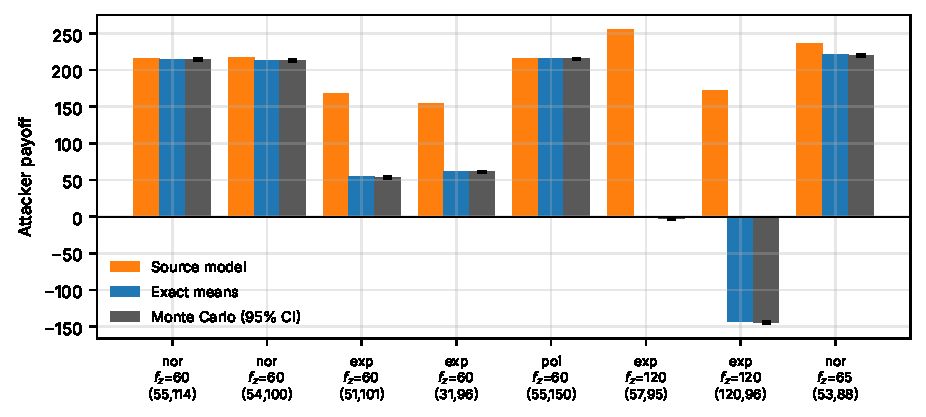
\includegraphics[width=0.85\textwidth]{fig_validation.pdf}
\caption{Attacker payoff at selected points: source model, exact-truncated-mean variant and flow-level simulation.}
\label{fig:val}
\end{figure*}

\subsection{Disagreement for exponential attackers}
For exponential attackers the picture is different at the tested points. At the source model's best subgame saddle for $f_z{=}60$, $(51,101)$, the model predicts 167.4 and the simulation gives $53.5\pm1.1$. At the source-model best subgame saddle for $f_z{=}120$, $(57,95)$, the model predicts 255.3 and the simulation gives $-2.7\pm1.3$. The component that differs is the attacker's bandwidth share: the model says 0.385 at the first point and the simulation says 0.278. This points to the admitted-traffic approximation as a major source of error for exponential traffic in these cases.

%==============================================================
\section{Exact Truncated First Moment}\label{sec:exact}

\subsection{The approximation}
The source model estimates the admitted mean rate of a flow as $f'=f\,\Pr(F\le M)$. The truncated first moment is
\begin{equation}
f'_{\text{trunc}}=\mathbb{E}\big[F\,\mathbf 1\{F\le M\}\big].
\end{equation}
For exponential traffic with mean $f$ and $r=M/f$ the two are
\begin{equation}
f\big(1-e^{-r}\big)\quad\text{versus}\quad f\big(1-e^{-r}(1+r)\big).
\end{equation}
At $f{=}120$ and $M{=}95$, so $r\approx0.79$, they are $0.547f$ and $0.189f$: the source formula overstates the admitted rate of an exponential attacker by about a factor of 2.9. The reason is that thresholding an exponential removes exactly the large values that carry most of its mean, so the surviving flows are much slower than the average. For a normal attacker with mean 60 and spread 20, a threshold of 100 or more lies at least two standard deviations above the mean and removes almost nothing, which is why the approximation is harmless there. Poisson attackers behave the same way. For normal and Poisson families we use
\begin{align}
\mathbb{E}[F\mathbf 1\{F\le M\}]_{\text{normal}} &= f\,[\Phi(b)-\Phi(a)]+\sigma\,[\varphi(a)-\varphi(b)],\\
\mathbb{E}[F\mathbf 1\{F\le M\}]_{\text{Poisson}} &= f\,\Pr(F\le\lfloor M\rfloor-1),
\end{align}
with $a=-f/\sigma$ (for rates clipped at zero), $b=(M-f)/\sigma$, and $\varphi$ the standard normal density. The Poisson expression assumes integer-valued rates and the inclusive firewall convention $F\le M$. We apply the corresponding truncated first moment to legitimate traffic as well.

\subsection{Effect on selected subgames}
Table~\ref{tab:sub2} compares the source and exact-truncated-mean variants at $f_z{=}60$; the last column gives the simulated payoff at the latter variant's subgame saddle. Across the eight selected points in Table~\ref{tab:val}, exact-truncated-mean payoffs differ from simulated means by less than two payoff points. This is a finite set of comparisons, not evidence of uniform agreement over the strategy grid. The correction changes the exponential subgame substantially: its best subgame saddle moves from 51 to 31 zombies and its payoff from 167.4 to 61.6.

\begin{table}[t]
\caption{Fixed-mean subgames at $f_z{=}60$: source and exact-truncated-mean variants, $(z^*,M^*,\text{payoff})$}
\label{tab:sub2}
\centering\scriptsize
\begin{tabular}{lccc}
\toprule
Family & Source model & Truncated means & Simulated at trunc. mean\\
\midrule
Normal & (55,114,215.3) & (54,100,213.0) & $212.9\pm1.0$\\
Exponential & (51,101,167.4) & (31,96,61.6) & $61.2\pm1.1$\\
Poisson & (55,150,215.4) & (55,150,215.2) & $215.5\pm0.8$\\
\bottomrule
\end{tabular}
\end{table}

\subsection{Effect on the nested subgame scan}
Within the nested scan, the exact-truncated-mean variant's highest-payoff exponential subgame saddle is 62.3 at $f_z{=}54$ ($z{=}32$, $M{=}97$), below the corresponding normal and Poisson values in Table~\ref{tab:general}. This family-wise ranking is a comparison of subgame saddles only; the full finite game has no pure saddle for either payoff variant (Table~\ref{tab:fullgame}). Fig.~\ref{fig:br} shows the attacker's best-response value against the threshold at $f_z{=}60$ for each family and variant. Fig.~\ref{fig:eq} shows the payoff at each available subgame saddle against the attacker's mean rate. In this nested comparison, the source-model exponential values rise to the largest reported subgame payoff, whereas its exact-truncated-mean values remain lower and lack a subgame saddle for 20 of the 120 scanned mean rates. These results do not establish which family is best in the combined game.

\begin{figure*}[t]
\centering
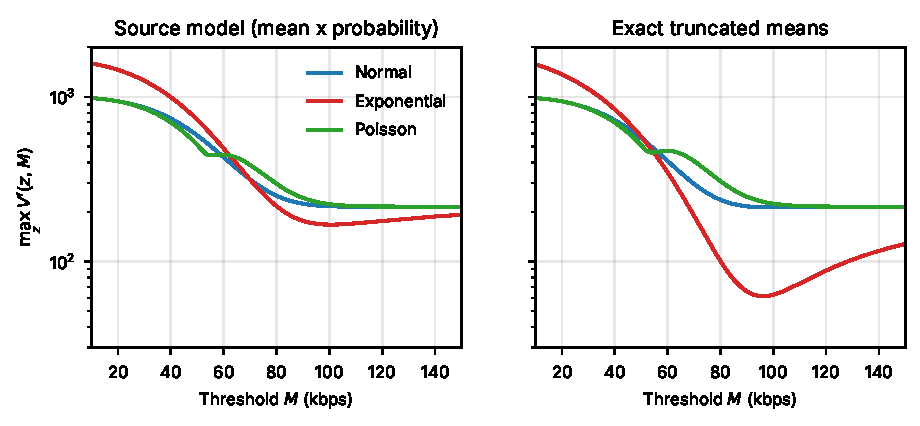
\includegraphics[width=0.85\textwidth]{fig_best_response.pdf}
\caption{Attacker's best-response value against the firewall threshold at $f_z{=}60$~kbps, under the source model (left) and the exact-truncated-mean variant (right). The defender's minimax threshold is where each curve is lowest.}
\label{fig:br}
\end{figure*}

\begin{figure*}[t]
\centering
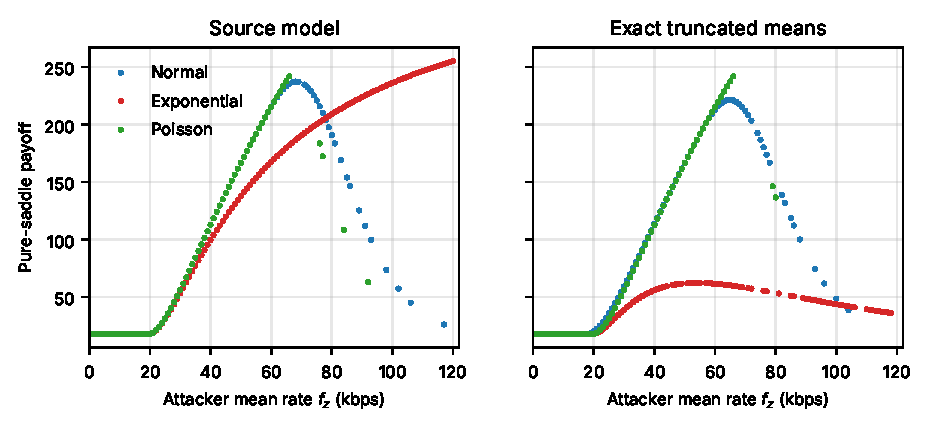
\includegraphics[width=0.85\textwidth]{fig_eq_vs_fz.pdf}
\caption{Payoff at each available fixed-parameter subgame saddle against the attacker's mean rate. Missing points have no pure saddle in that subgame. The family-wise comparison does not represent a combined-game equilibrium.}
\label{fig:eq}
\end{figure*}

%==============================================================
\section{Where the Threshold Should Sit}\label{sec:thr}
The attacker-side findings do not determine an equilibrium threshold for the combined simultaneous game. We instead report a finite-grid flow-level simulation for the case the original ns-2 study examined: a normal attacker with $f_z{=}60$~kbps.

On a sweep that copies the ns-2 grid ($z\in\{10,\dots,120\}$, $M\in\{10,\dots,140\}$~kbps) with 1000 replications per cell, the sample-mean payoff matrix has an apparent saddle at $(z,M){=}(50,100)$ with payoff 211.2. On a finer grid (steps of 5, 600 replications), the sample-mean matrix has an apparent saddle at $(55,95)$ with payoff 213.1. These locations are point estimates from finite simulations, not uncertainty-quantified equilibrium estimates. Fig.~\ref{fig:mc} shows the simulated payoff surface. The ns-2 study reports $z\approx50$, $M\approx90$~kbps and payoff about 170.6. Our threshold estimates lie between the ns-2 result and the source-model subgame results, and near the exact-truncated-mean normal subgame result. Our flow-level sample payoffs (about 211--213) are roughly 25\% higher than 170.6; without the original seeds and traces, we cannot attribute that difference to specific packet-level effects.

The attacker's global maximum on the coarse sweep is at the corner $(z,M){=}(10,10)$ with a payoff near 971. This is the situation of Remark~1: a firewall that rejects almost everyone hands the attacker the user-loss term. The defender's minimax threshold is the point on the attacker's best-response curve that avoids it.

\begin{figure}[t]
\centering
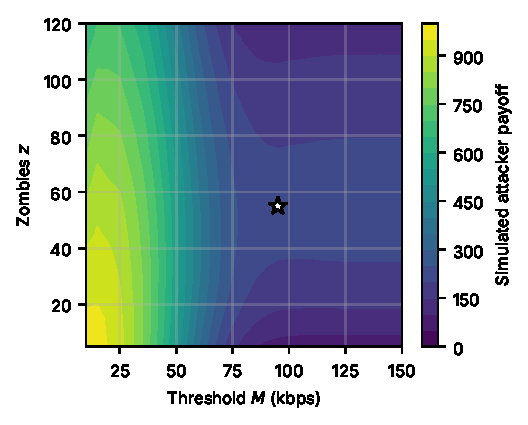
\includegraphics[width=0.85\columnwidth]{fig_mc_surface.pdf}
\caption{Flow-level sample-mean attacker payoff for a normal attacker at $f_z{=}60$~kbps. The star marks the apparent saddle on this finite sample and grid.}
\label{fig:mc}
\end{figure}

%==============================================================
\section{Sensitivity to the Payoff Weights}\label{sec:sens}
Because the weights are hypothetical, we varied $w_z$ and $w_u$ one at a time for the exact-truncated-mean normal subgame at $f_z{=}60$ (Table~\ref{tab:sens}).

\begin{table}[t]
\caption{Sensitivity of the exact-truncated-mean normal subgame ($f_z{=}60$), $(z^*,M^*,\text{payoff})$}
\label{tab:sens}
\centering\scriptsize
\begin{tabular}{lc}
\toprule
Weight changed & Equilibrium\\
\midrule
$w_z{=}2$ & (120 (grid edge), 91, 478.8)\\
$w_z{=}5$ (base) & (54, 100, 213.0)\\
$w_z{=}10$ & (16, 113, 55.8)\\
$w_z{=}20$ & (0, 150, 17.9)\\
\midrule
$w_u{=}500$ & (50, 86, 188.0)\\
$w_u{=}1000$ (base) & (54, 100, 213.0)\\
$w_u{=}2000$ & (64, 111, 255.2)\\
\bottomrule
\end{tabular}
\end{table}

The subgame saddle's fleet size is sensitive to the cost weight, in line with the $w_z^{-1/2}$ scaling suggested by~\eqref{eq:zstar}: halving the cost pushes the selected fleet to the edge of the searched range, and quadrupling it yields $z^*{=}0$. The payoff changes by a factor of more than 25 across the $w_z$ range. The threshold moves less, between 86 and 113~kbps over every non-degenerate case, which is a spread of about $\pm14$~kbps around the base value. These results describe sensitivity within the selected subgame, not a threshold recommendation for the combined game. Raising $w_u$ makes user loss matter more, so the attacker's fleet, the threshold and the payoff all rise. The same exercise on the source model for exponential traffic at $f_z{=}120$ shows the same pattern (fleet 19 to 120 across $w_z$, threshold 92 to 98).

%==============================================================
\section{Discussion}\label{sec:disc}

\subsection{What the model does well}
Its main merit is that it makes assumptions explicit. Because the payoff has three separable terms, it is possible to examine how each term affects fixed-parameter subgames. The sensitivity analysis shows that, within the selected normal subgame, changes in the hypothetical cost weight move the saddle fleet more than the threshold. This is a conditional property of the modeled subgame, not a robust threshold recommendation for the combined game.

\subsection{What the correction changes, and what it does not}
Within the nested subgame scan, replacing the mean-times-probability approximation with the exact truncated first moment sharply reduces the exponential-family saddle payoffs. Intuitively, an exponential attacker's traffic includes high-rate flows that contribute disproportionately to total bandwidth; a rate threshold removes those flows. The normal and Poisson fixed-mean subgames change much less in the tested cases. This correction changes the family-wise ranking of the nested subgame saddles, but the full-grid calculation shows that neither variant has a pure saddle in the combined game. We therefore cannot infer from these subgame rankings which distribution is optimal for the attacker when the defender chooses a single threshold simultaneously.

This should be read with care. The conclusion applies to the model as we read it. We do not have the original Matlab code, and the original authors may have used a different expression for the exponential case. We therefore frame it as a result about the mean-times-probability rule rather than as a claim about the authors' implementation. We have not contacted them, and doing so is the first item of future work.

\subsection{How to read the original numbers}
The original paper reports fixed-mean subgame outcomes, a general-game result, and a simulated optimum. They come from different procedures and should not be treated as competing estimates of one quantity. Our nested scan reproduces the fixed-mean subgames and compares its highest-payoff subgame saddles with the reported general-search values; it does not establish a pure equilibrium of the combined game. The ns-2 study uses a normal attacker, so it provides evidence about the normal $f_z{=}60$ case, not about the exponential-family result.

\subsection{Toward operational use}
An operator seeking to use this framework would need to estimate legitimate rates from measurements, define the modeled ``user'' (flow, session or customer), calibrate the weights, and decide where to place the filter. Since the full finite game has no pure saddle on the grid tested here, a worst-case threshold analysis would also need to account for mixed strategies or adopt a different move order. These results alone do not provide an operational threshold.

\subsection{Threats to validity}
Our implementation is an interpretation: the article does not give explicit expressions for the exponential and Poisson cases, all grid details, or the tie-breaking rule, and we resolved these ourselves. The choice of 20~kbps for the spread was selected because it reproduces the published payoff scale; it is not independently confirmed. The flow-level simulator shares our fair-sharing assumption and clips normal rates at zero, so it checks the expectation arithmetic under our modeled network rather than validating a packet-level network model. The Monte Carlo results use fixed seeds and finite replications. We report confidence intervals for selected payoff comparisons, but not uncertainty intervals for the sample-mean saddle locations. Finally, the combined-game check fixes the normal spread at 20~kbps and does not include the varied-spread normal actions reported in the nested scan.

%==============================================================
\section{Limitations and Future Work}\label{sec:limits}
\textbf{Model.} The game is one-shot and assumes a perfectly rational attacker, although real attackers adapt, probe and miscalculate. The zero-sum assumption ignores that defence has its own costs, such as extra compute, paid upstream capacity and support load, and that the attacker may value disruption differently from the payoff terms. Flows are constant-rate UDP, the legitimate population is homogeneous, the topology has one bottleneck, and the attacker's distribution family is small and fixed in advance. Rate is a weak signal of intent: a flash crowd of honest users and a low-and-slow attack both defeat a pure rate rule. The payoff weights are hypothetical.

\textbf{This paper.} Our simulation is flow-level and does not replace ns-2. We did not compare the hard threshold with the sigmoid rule. We tested only the parameter set of the original study. The exact-truncated-mean variant removes one approximation, but the additive loss formula~\eqref{eq:VU} remains in the analytical model, and we have not studied its effect separately. We have not computed mixed-strategy equilibria for the combined game.

\textbf{Future directions.} In the order we would attempt them:
\begin{itemize}
\item contact the original authors, or reconstruct their search, to explain the gap between 331.1 and our 172.7 for the published configuration;
\item compute mixed-strategy equilibria for the combined finite game and quantify uncertainty in the simulated subgame saddle locations;
\item replicate the ns-2 experiment with multiple seeds, common random numbers and confidence intervals, and extend it to exponential and Poisson attackers;
\item validate the legitimate-traffic assumption against real traces, such as the CAIDA datasets the original authors mention;
\item replace the zero-sum payoff with separate attacker and defender utilities and move to repeated or Stackelberg play, which would let the defender commit to a threshold first;
\item combine the external-attacker model with insider-threat models and with economic factors such as attack cost versus defence cost and the value of the protected service.
\end{itemize}

%==============================================================
\section{Conclusion}\label{sec:concl}
We independently implemented a one-shot firewall-threshold model and compared its fixed-parameter subgames with reported results and selected flow-level simulations. The fixed-mean subgame values are close to those published, but we could not reproduce the reported general-search value of 331.1. Correcting the mean-times-probability approximation substantially changes exponential-traffic subgame payoffs; the exact-truncated-mean variant agrees with simulation to within two payoff points at the eight parameter points tested. These findings are conditional on our interpretation and parameter choices. Crucially, a full-grid maximin/minimax check finds no pure-strategy saddle for either payoff variant in the combined simultaneous game, and we have not computed the mixed-strategy equilibria. The results therefore support further study of the model and its assumptions, not a definitive attacker-family ranking or an operational threshold recommendation.

%==============================================================
\section*{Acknowledgment}
We thank our course instructors for guidance on the project.

%==============================================================
\begin{thebibliography}{99}
\bibitem{spyridopoulos2013}
T.~Spyridopoulos, G.~Karanikas, T.~Tryfonas, and G.~Oikonomou, ``A game theoretic defence framework against {DoS/DDoS} cyber attacks,'' \emph{Comput.\ Secur.}, vol.~38, pp.~39--50, 2013, doi:10.1016/j.cose.2013.03.014.

\bibitem{wu2010}
Q.~Wu, S.~Shiva, S.~Roy, C.~Ellis, and V.~Datla, ``On modeling and simulation of game theory-based defense mechanisms against {DoS} and {DDoS} attacks,'' in \emph{Proc.\ 2010 Spring Simulation Multiconference (SpringSim '10)}, 2010, pp.~159:1--159:8.

\bibitem{dingankar2007}
C.~Dingankar and R.~R. Brooks, ``Denial of service games,'' in \emph{Proc.\ 3rd Annu.\ Cyber Security and Information Infrastructure Research Workshop}, 2007, pp.~7--17.

\bibitem{fallah2010}
M.~Fallah, ``A puzzle-based defense strategy against flooding attacks using game theory,'' \emph{IEEE Trans.\ Dependable Secure Comput.}, vol.~7, no.~1, pp.~5--19, 2010.

\bibitem{walfish2006}
M.~Walfish, M.~Vutukuru, H.~Balakrishnan, D.~Karger, and S.~Shenker, ``{DDoS} defense by offense,'' in \emph{Proc.\ ACM SIGCOMM}, 2006, pp.~303--314.

\bibitem{li2009}
J.~Li, N.~Li, X.~Wang, and T.~Yu, ``Denial of service attacks and defenses in decentralized trust management,'' \emph{Int.\ J.\ Inf.\ Secur.}, vol.~8, pp.~89--101, 2009.

\bibitem{mirkovic2004}
J.~Mirkovic and P.~Reiher, ``A taxonomy of {DDoS} attack and {DDoS} defense mechanisms,'' \emph{ACM SIGCOMM Comput.\ Commun.\ Rev.}, vol.~34, no.~2, pp.~39--53, 2004.

\bibitem{zargar2013}
S.~T. Zargar, J.~Joshi, and D.~Tipper, ``A survey of defense mechanisms against distributed denial of service ({DDoS}) flooding attacks,'' \emph{IEEE Commun.\ Surveys Tuts.}, vol.~15, no.~4, pp.~2046--2069, 2013.

\bibitem{manshaei2013}
M.~H. Manshaei, Q.~Zhu, T.~Alpcan, T.~Ba\c{s}ar, and J.-P. Hubaux, ``Game theory meets network security and privacy,'' \emph{ACM Comput.\ Surv.}, vol.~45, no.~3, art.~25, 2013.

\bibitem{vonneumann1928}
J.~von Neumann, ``Zur Theorie der Gesellschaftsspiele,'' \emph{Math.\ Ann.}, vol.~100, pp.~295--320, 1928.

\bibitem{nash1951}
J.~Nash, ``Non-cooperative games,'' \emph{Ann.\ Math.}, vol.~54, no.~2, pp.~286--295, 1951.

\bibitem{osborne1994}
M.~J. Osborne and A.~Rubinstein, \emph{A Course in Game Theory}. Cambridge, MA, USA: MIT Press, 1994.
\end{thebibliography}

\end{document}
